\section{Ergebnisse}
\autor{Felix Anslinger}

Die Formel zur Berechnung der Vorschauweite wurde durch eine Python Simulation verifiziert. \cite{vorschauweite_notebook}

Durch die Implementierung des Stanley-Controllers in einer MATLAB/Simulink Umgebung, mittels der in Kapitel 4.3 beschriebenen Formeln, lässt sich die Performance des Reglers testen. Die Simulation umfasst nicht nur die Stanley-Regelformel, sondern bezieht auch eine simulierte Totzeit sowie die entsprechende Berechnung der, in Kapitel 4.3.4 beschriebenen, Vorschauweite mit ein. Das Ergebnis der Simulation ist in Abbildung \ref{fig:stanley_matlab_simulationsergebniss} dargestellt, wobei die gestrichelte blaue Linie die Solltrajektorie und die rote Linie die Fahrstrecke des Fahrzeugs abbilden.

\begin{figure}[H]
    \centering
    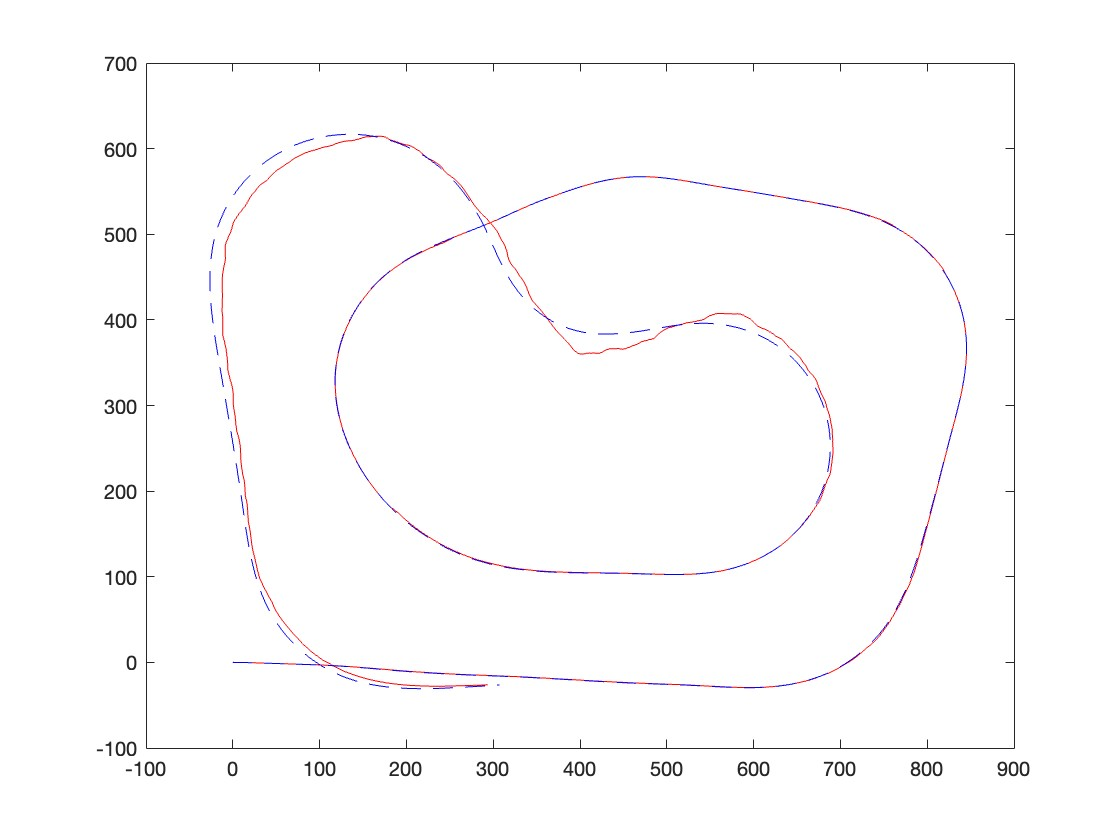
\includegraphics[width=1\linewidth]{Pictures/stanley_controller_performance_matlab.jpg}
    \caption{Stanley-Regler in MATLAB Simulation}
    \label{fig:stanley_matlab_simulationsergebniss}
\end{figure}

 Das Ergebnis aus Abbildung \ref{fig:stanley_matlab_simulationsergebniss} zeigt, dass der Stanley-Regler stabil ist und somit kein instabiles Aufschwingen auftritt. Des Weiteren lässt sich bei diesem Regler keine anhaltende Regelabweichung feststellen.


%\section{Ausblick}